\documentclass[a4paper, 10pt]{article}

\usepackage[utf8]{inputenc}
\usepackage[english]{babel}
\usepackage[T1]{fontenc}
\usepackage{lmodern}
\usepackage[width=15.50cm, height=22.00cm]{geometry}
\usepackage{amsmath}
\usepackage{amssymb}
\usepackage{amsthm}
\usepackage{esdiff}
\usepackage{url}
\usepackage{listings}
\usepackage{color}
\usepackage{graphicx}
\usepackage{epstopdf}
\usepackage{subcaption}
\usepackage{caption}

\definecolor{mygreen}{rgb}{0,0.6,0}
\definecolor{mygray}{rgb}{0.5,0.5,0.5}
\definecolor{light}{rgb}{0.96, 0.96, 0.96}
\definecolor{mymauve}{rgb}{0.58,0,0.82}

\lstset{ %
	backgroundcolor=\color{light},   % choose the background color; you must add \usepackage{color} or \usepackage{xcolor}
	basicstyle=\footnotesize,        % the size of the fonts that are used for the code
	breakatwhitespace=false,         % sets if automatic breaks should only happen at whitespace
	breaklines=true,                 % sets automatic line breaking
	captionpos=b,                    % sets the caption-position to bottom
	commentstyle=\color{mygreen},    % comment style
	deletekeywords={},            	 % if you want to delete keywords from the given language
	escapeinside={\%*}{*)},          % if you want to add LaTeX within your code
	extendedchars=true,              % lets you use non-ASCII characters; for 8-bits encodings only, does not work with UTF-8
	frame=single,	                 % adds a frame around the code
	keepspaces=true,                 % keeps spaces in text, useful for keeping indentation of code (possibly needs columns=flexible)
	keywordstyle=\color{blue},       % keyword style
	language=C++,                    % the language of the code
	otherkeywords={},           	 % if you want to add more keywords to the set
	numbers=left,                    % where to put the line-numbers; possible values are (none, left, right)
	numbersep=5pt,                   % how far the line-numbers are from the code
	numberstyle=\tiny\color{mygray}, % the style that is used for the line-numbers
	rulecolor=\color{black},         % if not set, the frame-color may be changed on line-breaks within not-black text (e.g. comments (green here))
	showspaces=false,                % show spaces everywhere adding particular underscores; it overrides 'showstringspaces'
	showstringspaces=false,          % underline spaces within strings only
	showtabs=false,                  % show tabs within strings adding particular underscores
	stepnumber=1,                    % the step between two line-numbers. If it's 1, each line will be numbered
	stringstyle=\color{mymauve},     % string literal style
	tabsize=3,	                     % sets default tabsize to 2 spaces
	title=\lstname                   % show the filename of files included with \lstinputlisting; also try caption instead of title
}

\setlength{\parindent}{0 cm}
\setlength{\parskip}{0 cm}
\pagenumbering{arabic}
\frenchspacing
\selectlanguage{english}

\newtheorem{mydef}{Definition}
\newcommand{\horrule}[1]{\rule{\linewidth}{#1}}
\newcommand{\includecode}[2][c]{\lstinputlisting[caption=#2, escapechar=, style=custom#1]{#2}<!---->}
\newcommand{\norm}[1]{\lVert#1\rVert}
\newcommand{\abs}[1]{\lvert#1\rvert}
\renewcommand{\vec}[1]{\mathbf{#1}}
\newcommand*\colvec[3][]{
	\begin{pmatrix}\ifx\relax#1\relax\else#1\\\fi#2\\#3\end{pmatrix}
}

\title{\horrule{0.5 pt}\\[0.4cm] \textbf{High Performance Computing \\ for Mathematical Models} \\ {\large 2D Fluid Solver} \horrule{1 pt}}
\author{Jan Kirchner, Petr Valenta}
\date{\today}

\begin{document}

\maketitle
{\small This document is a part of the assessment work for the subject WMMS5311 High Performance Computing for Mathematical Models lectured at ENSIMAG, Grenoble INP.}

\begin{abstract}
	This document describes a 2D fluid flow solver. The code is written in \texttt{C++} programming language and parallelized using \texttt{MPI} library. The mathematical description of the flows as well as the implementation and parallelization of the code is briefly discussed. In the last part, the results of several performance tests are presented. All source files can be found at \url{https://github.com/valenpe7/2d_fluid_solver}.  
\end{abstract}

\tableofcontents

\section{Introduction}
For the final project of the course "High performance computing for mathematical models" we had to apply the methods we learned during the course to parallelize a numerical application that we developed in a previous course using \texttt{MPI}\textsuperscript{\cite{gabriel04:_open_mpi}} library. In this report we are going to explain how to use the final program, how we parallelized it and how the parallelization influenced the performance of the program. We chose to work with fluid solver that computes the solution to the 2D incompressible Navier-Stokes equations for a specified fluid in a specified environment to acquire values for the velocity and the pressure of the fluid at the respective positions in the environment.\\

The implementation of the solver as well as the mathematical exposition of the problem in this report follows Griebel \textsuperscript{\cite{Griebel:1998:NSF:280492}}. At the core of the program in the method \texttt{solve\_Poisson\_Jacobi()} the relaxed Jacobi method is used to approximate a solution for the Poisson equation. The Jacobi method is a classic example for a method that can be efficiently parallelized and that is the reason why we chose this program. We decided furthermore to rewrite the complete program to include \texttt{MPI} to improve performance further.\\

\begin{figure}
	\centering
	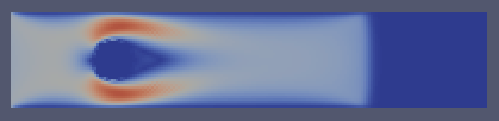
\includegraphics[scale=0.7]{img/1.png}
	\caption{One sample evaluation of the fluid solver at one time step.}
\end{figure}

\section{Implementation}
The behavior of incompressible flows is described by the well known Navier-Stokes equations:
\begin{equation}
\label{1}
\frac{\partial}{\partial t}\vec{u} + (\vec{u} \cdot \text{grad})\vec{u} + \textrm{grad}p =\frac{1}{Re}\Delta\vec{u}+\vec{g} \qquad \textrm{(momentum equation)},
\end{equation}
\begin{equation}
\label{2}
\textrm{div}\vec{u} = 0 \qquad \textrm{(continuity equation)}.
\end{equation}
where $ t > 0 $ denotes time, $ \vec{u} $ is the velocity field, $p$ is the pressure, $ Re $ is the Reynolds number and $ \vec{g} $ denotes body forces such as gravity acting throughout the bulk of the fluid. When solving the 2D case of the system (\ref{1}), (\ref{2}) discretized in time with time step $ \Delta t $, the following \textit{Poisson equation for the pressure} $p^{(n+1)}$ arises:
\begin{equation}
\label{3}
\frac{\partial^2p^{n+1}}{\partial x^2} + \frac{\partial^2p^{n+1}}{\partial y^2} = \frac{1}{\Delta t}\Big(\frac{\partial F^{n}}{\partial x} + \frac{\partial G^{n}}{\partial y}\Big),
\end{equation}
where
\begin{equation*}
F^{n} = u_x^{n} + \Delta t \left[ \frac{1}{Re}\left( \partial_x^{2} u_x^n + \partial_y^{2} u_y^n \right) - \partial_x (u_x^2)^n - \partial_y (u_x u_y)^n + g_x \right],  
\end{equation*}
\begin{equation*}
G^{n} = u_y^{n} + \Delta t \left[ \frac{1}{Re}\left( \partial_x^{2} u_y^n + \partial_y^{2} u_x^n \right) - \partial_y (u_y^2)^n - \partial_x (u_x u_y)^n + g_y \right].
\end{equation*}
The equation (\ref{3}) can reliably be solved with the \textit{Jacobi relaxation method}. To achieve the standard form of the equation, first the right hand side of the equation is computed at each grid point and time step. The update of the pressure then occurs in the method \texttt{solve\_Poisson\_Jacobi()} according to the updating formular:
\begin{equation*}
p_{i,j}^{\textnormal{it}+1} := (1-\omega)p_{i,j}^{\textnormal{it}} + \frac{\omega}{\frac{\varepsilon_i^E + \varepsilon_i^W}{\Delta x^2} + \frac{\varepsilon_j^N + \varepsilon_j^S}{\Delta y^2}} \left( \frac{\varepsilon_i^Ep_{i+1,j}^{\textmd{it}} + \varepsilon_i^Wp_{i-1,j}^{\textmd{it}}}{\Delta x^2}+\frac{\varepsilon_i^Np_{i,j + 1}^{\textmd{it}} + \varepsilon_i^Sp_{i, j-1}^{\textmd{it}}}{\Delta y^2} - \mathrm{RHS}_{i,j}\right)
\end{equation*}
for $ i = 1 , \dots, i_{\max} $ and $ j = 1, \dots, j_{\max} $, where $\omega\in(0, 1)$ and the parameters $ \varepsilon \in \{0, 1\} $ indicate whether cell $ (i, j) $ lies adjacent to the domain boundary. The superscripts
W, E, N, and S indicate in which direction (west, east, north, or south) the boundary lies. These updates are repeated until convergence is achieved. These computations are the most expensive part of the solver and parallelizing them should significantly increase the code performance.\\

We chose to consider the problem column-wise, thus the domain is divided into columns and workload is distributed between individual processes accordingly. In our version of code, the number of processes has to be divisor of the number of cells in the horizontal direction. Wherever during computation quantity relies on values from the neighboring columns, information is exchanged between the processes using \texttt{MPI} library routines.

\section{Compilation and executing}

For the compilation, one can use the attached bash script "compile" which executes prepared makefile. Due to the usage of features introduced by the latest revision of C++ standards, the minimum required version of GCC is 4.8.\\

To execute the fluid solver, a \texttt{.png} file is required to specify the environment \footnote{Obstacles in the environment are specified via the alpha channel of the prepared \texttt{.png} file. The value 0 indicates an empty field, while any other value indicates an obstacle.}. Compiled application takes the filename of the input image and output path for the exported \texttt{.vtk} files as an argument. Other parameters like fluid properties, the geometry of the simulation domain, boundary conditions, etc. can be specified in the code before the compilation. The  \texttt{.vtk} files can be displayed with a software tools such as \texttt{ParaView} or \texttt{VisIt}. \\

\section{Results}
As a part of the project, several performance test were done on a clusters operated and managed by Czech National Grid Organization MetaCentrum. We chose cluster minos.zcu.cz, which contains 50 nodes, each of the nodes has the following hardware specification:

\begingroup
\renewcommand*{\arraystretch}{1.5}
\begin{table}[h!]
	\centering
	\begin{tabular}{ | c | l | }
		\hline
		CPU & 2 $ \times $ 6-core Intel$ ^{{\scriptsize \textregistered}} $ Xeon$ ^{{\scriptsize \textregistered}} $ E5645 2.40 GHz \\ \hline
		RAM & 24 GB \\ \hline
		Disk & 2 $ \times $ 600 GB \\ \hline
		Net & 1 Gbit/s Ethernet, Infiniband. IB switches of clusters are connected by 6 $ \times $ 40Gb/s \\ \hline
		Owner & CESNET \\
		\hline
	\end{tabular}
	\caption{Specification of used computational resources}
	\label{2.3.16}
\end{table}
\endgroup

We made a model scene of size $ 1600 \times 400 $ cells with obstacles created using image, which is shown in Figure (2). The flow is coming from the north to the south boundary, in order to distribute workload between processes equivalently, since we have domain divided in columns. The temporary solution of exporting data from all processes into one \texttt{.vtk} file for visualization purposes is turned off during the performance tests, because significantly influences the computational time. The results of performed simulations can be seen in the Table (2).\\

From the measured times we calculated a speedup. The result is shown in Figure (3). It can be clearly seen, that up to 4 processes we achieved almost linear speedup. With the increase of the number of computational units, the value of speedup grows more slowly. Using more than 64 processors is inefficient in this case. The computational domain is too small, and thus the more time is spent for the communication between processes.

\begin{figure}[h!]
	\centering
	\fbox{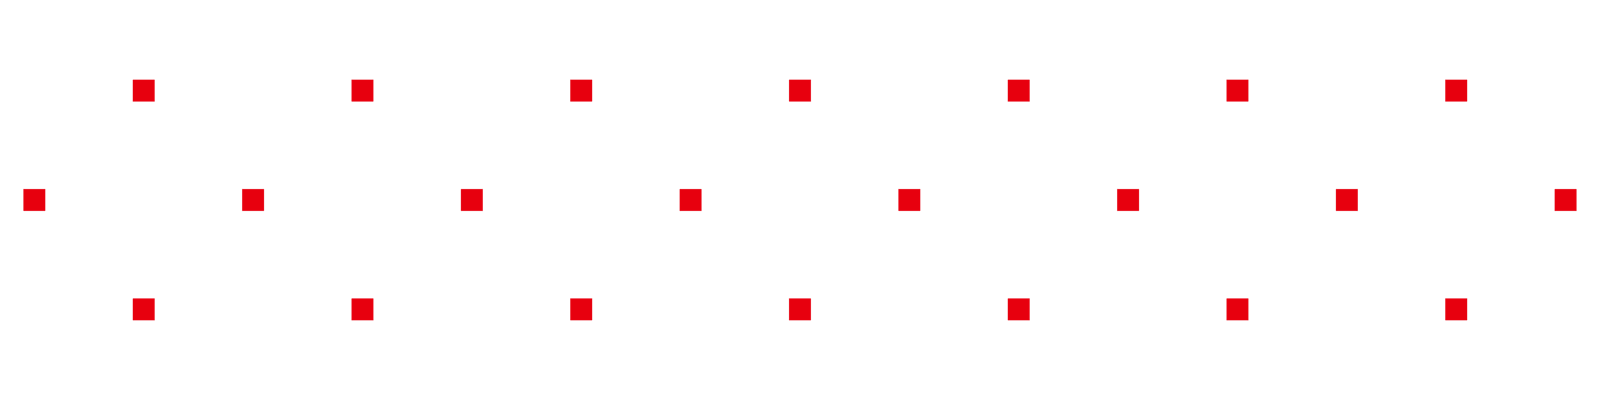
\includegraphics[width=0.7\linewidth]{img/3.png}}
	\caption{\texttt{.png} image of size $ 1600 \times 400 $ used for creating model scene for the performance tests of the code. Red squares are obstacles.}
\end{figure}

\begingroup
\renewcommand*{\arraystretch}{1.5}
\begin{table}[h!]
	\centering
	\begin{tabular}{  c | c | c }
		P & $ T_{total} $ (s) & $ T_{calcul} $ (s) \\
		\hline \hline
		1 & 415 & 404 \\ \hline
		2 & 208 & 202 \\ \hline
		4 & 123 & 112 \\ \hline
		8 & 87 & 74 \\ \hline
		16 & 55 & 42 \\ \hline
		32 & 31 & 23 \\ \hline
		64 & 23 & 13 \\ \hline
		80 & 32 & 12 \\
	\end{tabular}
	\caption{Total duration ($ T_{total} $) and duration of calculation without setup and completion ($ T_{calcul} $) of simulations according to the number of processors $ P $ on which had been executed.}
	\label{2.3.16}
\end{table}
\endgroup

\begin{figure}[h!]
	\centering
	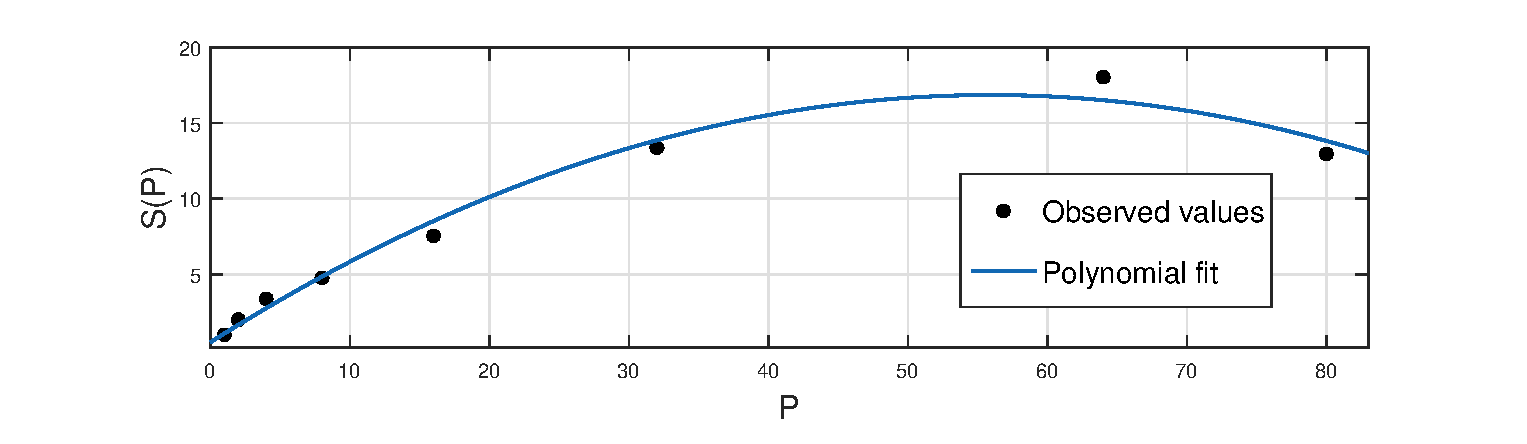
\includegraphics[width=0.9\linewidth]{img/2.eps}
	\caption{Speedup S(P) of the code depending on the number of processes P.}
\end{figure}


\section{Conclusion}

Even though the results of parallelization indicates significant improvement of the code, there is definitely still a lot of work to do. First, the domain should be divided into sub-domains not only in the x-direction, but also in the y-direction, to be sure, that the workload is distributed correctly independently of the fluid flow direction. Afterwards, we should handle the situation, when the number of cells is not divisor of the chosen number of processors. The next step should be rewriting of the routine for exporting the data. Current approach is inefficient and for the parallel computing completely useless. It has been used only to check if the solver works correctly in the parallel regime. The option could be exporting into parallel \texttt{.vtk} files.\\

{\bf \noindent Acknowledgements} \\

Authors would like to thank Mr. Christophe Picard, for the guidance and valuable advice he has provided throughout the course.\\

Access to computing and storage facilities owned by parties and projects contributing to the National Grid Infrastructure MetaCentrum, provided under the programme "Projects of Large Infrastructure for Research, Development, and Innovations" (LM2010005), is greatly appreciated.\\

Access to the CERIT-SC computing and storage facilities provided under the programme Center CERIT Scientific Cloud, part of the Operational Program Research and Development for Innovations, reg. no. CZ. 1.05/3.2.00/08.0144, is greatly  appreciated.\\
\begin{flushright}
	Jan Kirchner, Petr Valenta
\end{flushright}

\bibliographystyle{plain}
\bibliography{bib}

\end{document}